\section{Overview}\label{sec:overview}
The objective of this chapter is to provide our solution to transform Mirabilandia into a Micro City analyzing the requirements, the technologies and providing concrete solutions.

We will illustrate an architecture with all the components needed to satisfy the characteristics of an amusement park as a Micro City: offer a tailored and dynamic experience based on visitors' preferences and a situated recommendation system (Section~\ref{sec:requirements}) with a rewards system.

The goal of the architecture section is to define a way to keep track of visitors' position within the park, provide a recommendation and reward system, a way to smartly manage queues and visitors' information as well as provide a customizable plan of a day in the park.

As per the recommendation and reward systems, is important to point out their tightly coupled relationship since every suggested action provides some kind of recompense.
In ~\ref{tab:actions-rewards} are listed some examples of this relationship.

\begin{longtable}{|l|l|}
	\hline
	\textbf{Action}                                  & \textbf{Reward}                      \\
	\hline
	This show is starting in 5 minutes  & You can get a reserved seat in the front row \\
	\hline
	If you go to this roller coaster    & You can get a reduced queueing waiting time           \\
	\hline
	If you go to this shop              & You can get a discount on t-shirts           \\
	\hline
	Throw the plastic bottle in a smart bin & You can get a coin for the arcade            \\
	\hline
	\caption{Possible actions within Mirabilandia as a Micro City and their respective reward.}
	\label{tab:actions-rewards}
\end{longtable}

\section{Overall architecture}\label{sec:mira-microcity}

Finally, we will discuss possible deployment techniques in the park environment. 

\section{Overall architecture}\label{sec:mira-microcity}
Following the analysis of the ``as-is'' system and the goals set to adapt the Micro-City concept to Mirabilandia,
figure~\ref{fig:architecture-overview} shows the component diagram that models the entities involved and the main relationships between them.

The main components of the system are the following:

\begin{itemize}
	\item \textit{Map Manager:} is responsible for tracking the guest within the park and providing information about the current position
	\item \textit{Virtual Queueing System:} is responsible for managing the virtual queue for each attraction
	\item \textit{Recommendation System:} is responsible for providing recommendations to the visitors based on different factors that will be further discussed in the next sections.
	\item \textit{Planner:} is responsible for planning the itinerary of the guests based on their preferences and crowding of rides
	\item \textit{Visitor Manager:} is responsible for the management of the users' information, preferences and tickets selling
\end{itemize}

\begin{figure}[H]
	\centering
	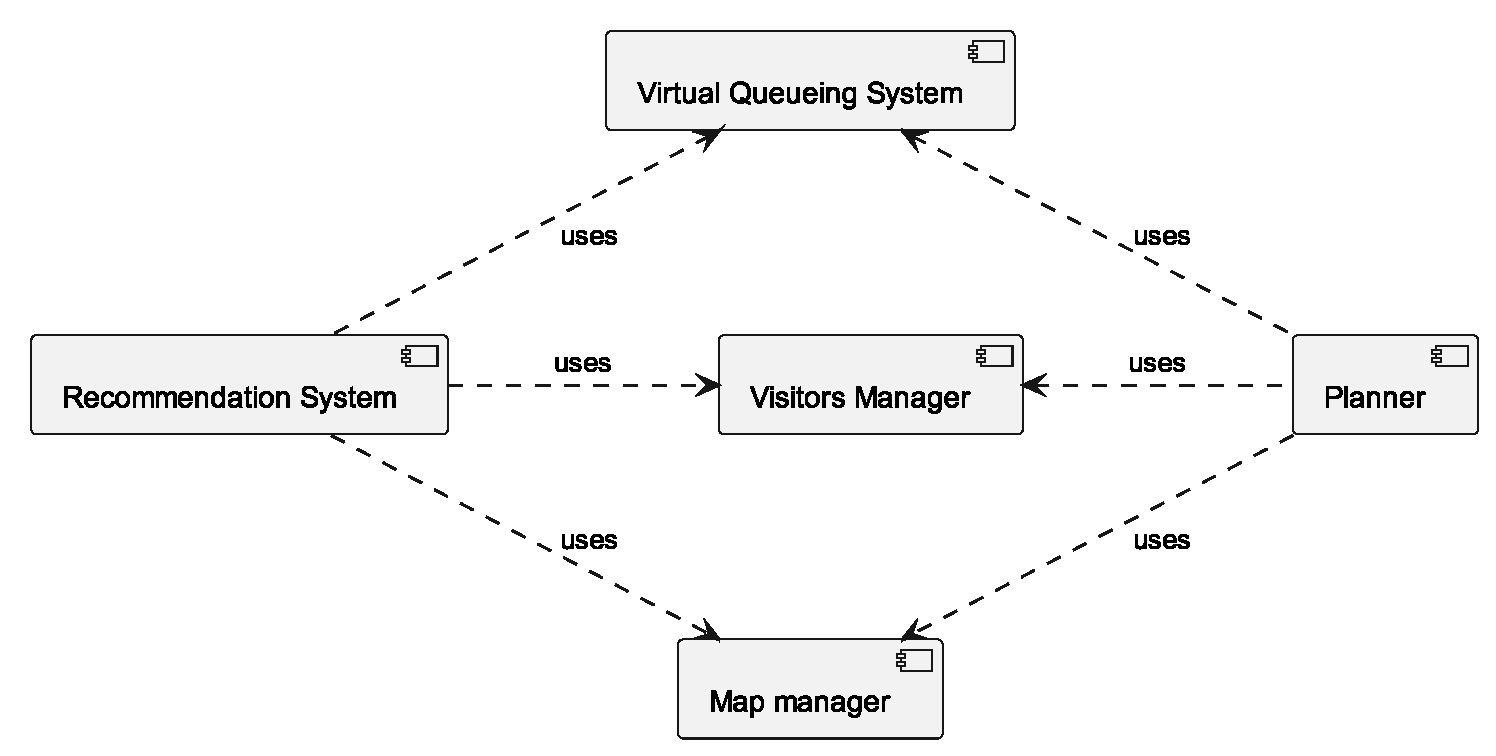
\includegraphics[width=0.9\textwidth]{img/architecture-overview.eps}
	\caption{Overall architecture of the Mirabilandia Micro-City.
		The Component Diagram shows the rough architecture and the main dependencies between the elements.
	}
	\label{fig:architecture-overview}
\end{figure}

From the diagram emerge that \textit{Map Manager} and \textit{Virtual Queueing System} are the main components of the system since they are the ones
that provide information to the other components. The \textit{Map Manager} provides information about the current position of the guests to the
\textit{Recommendation System} which uses this information to provide recommendations to the guests. Moreover, gives information also to the
\textit{Planner} to avoid crowd situations and maintain a uniform distribution of guests in the park. The \textit{Virtual Queueing System} is used by
the \textit{Planner} to plan the itinerary of the guests and adapt it to reduce the waiting time and improve the quality of the visit within the park
and by the \textit{Recommendation System} to fetch information about the current waiting time of the attractions and opportunistically advise the
attraction. The \textit{Visitor Manager} provides information to the \textit{Recommendation System} and the \textit{Planner} regarding users'
preferences.

\section{Map Manager}

The location of guests within the amusement park is critical for several reasons: guest location information is used to make recommendations and to
determine the best plan for each guest. So, good tracking is crucial for the good working of the overall system.

The \textit{Map Manager} component is composed of the following elements:
\begin{itemize}
	\item \textit{Device Information Ingestion:} is responsible for receiving, from the guests' devices, information that can be used to estimate the
	      current location of the guests. This component is the entry point of the \textit{Map Manger}.
	\item \textit{Location Inference:} is responsible for calculating the position of the guests based on the information received from the
	      \textit{Device Information Ingestion} component. This component leverage \textit{Location Data} to calculate the position of the guests.
	      Finally, this component exposes an interface to expose the current position of the guests to other components requiring information about
	      guests' positions within the park.
\end{itemize}

The figure~\ref{fig:map-manager} shows the component diagram that models the \textit{Map Manager} internal architecture.

\begin{figure}[H]
	\centering
	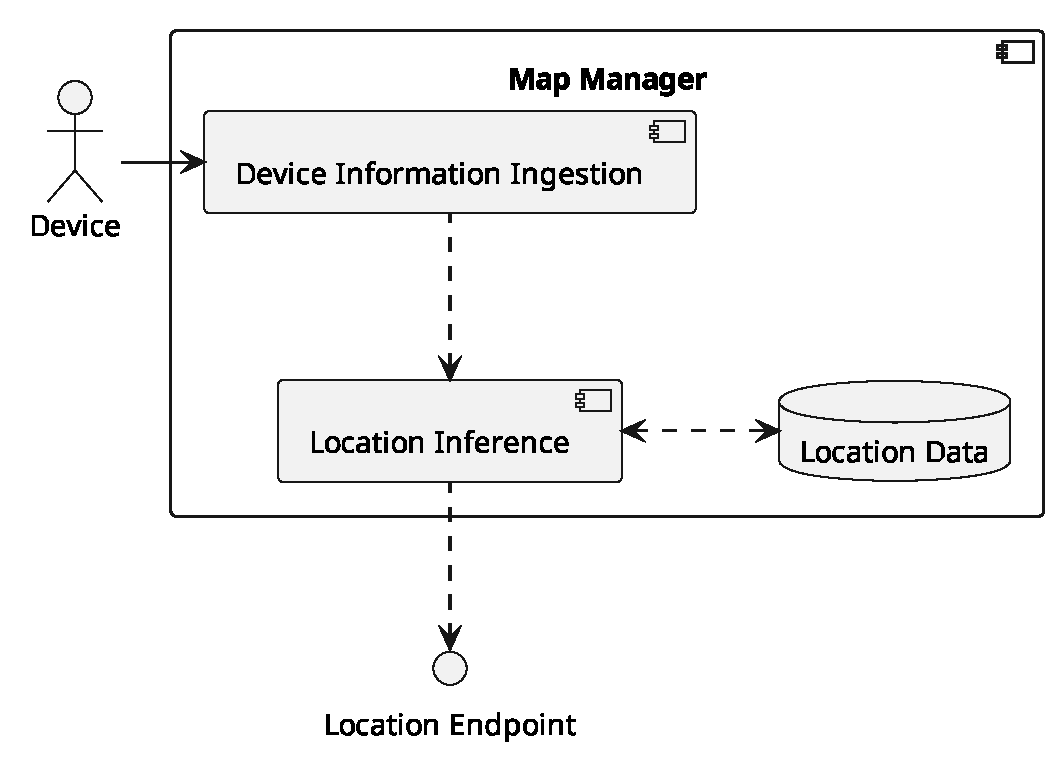
\includegraphics[width=0.7\textwidth]{img/map-manager-overview.eps}
	\caption{Component diagram showing the internal architecture of the \textit{Map Manager} component.}
	\label{fig:map-manager}
\end{figure}

Given the importance of this component and the amount of work it will have to do, attention must be paid to aspects of high availability to prevent
this component from stopping working since the operation of other services depends on it.

\section{Recommendation System}

\begin{figure}[H]
	\centering
	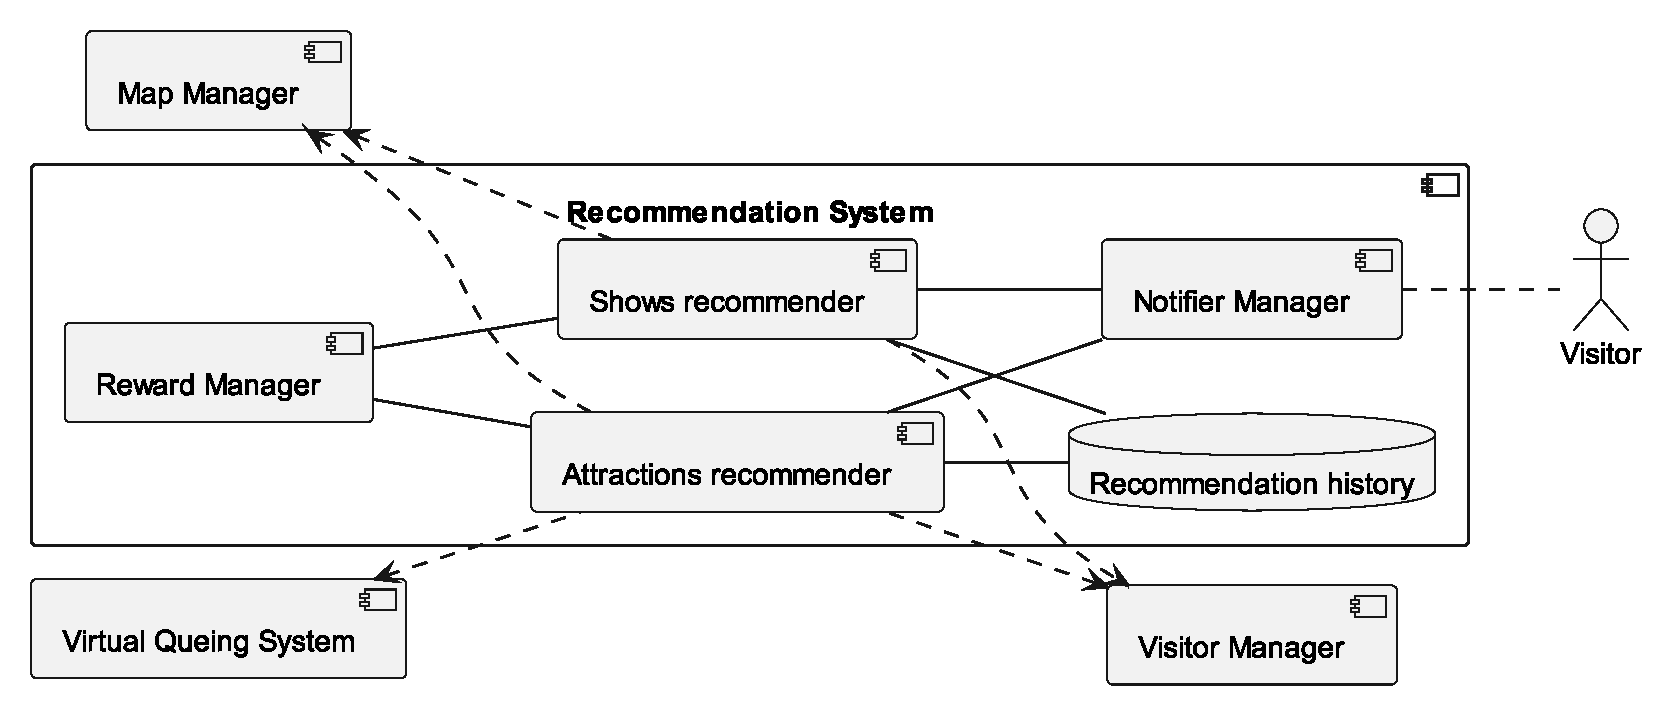
\includegraphics[width=\textwidth]{img/recommender.eps}
	\caption{Component diagram showing the internal architecture of the \textit{Recommender System}.
	}
	\label{fig:recommender-arch}
\end{figure}

The Recommendation System is a crucial component to ensure the improvement of the visitors' experience. In fact, it is responsible for collecting
data and providing tailored recommendations to the visitors and uses a Reward System to provide rewards based on the suggested actions. The Recommendation System is composed of:
\begin{itemize}
	\item \textit{Reward Manager} has access to all the rewards available to be given to visitors for a given recommendation. It works as displayed in figure~\ref{fig:reward}.
	      The visitors will receive a reward for the suggestions they take.
	\item \textit{Notification Manager} which sends the recommendation to the visitor's wearable.
	\item \textit{Shows Recommender} and \textit{Attractions Recommender} take visitor's information from the Visitor Manager to get their pre-compiled preferences.
	      In the former case, the subject would be a shows they are interested in, in the latter their preferred roller coasters, shops, etc. They also get the visitors' location from the Map Manager in order to make a recommendation based on their proximity to a point of interest (\textit{situated} recommendations).
	      In addition, the Attractions Recommender uses the Virtual Queueing System data, to provide recommendations also considering the waiting time of the attractions.
	\item \textit{Recommendation History} is responsible for storing the recommendations in order to improve the accuracy.
\end{itemize}

\section{Virtual Queuing System}
\begin{figure}[H]
	\centering
	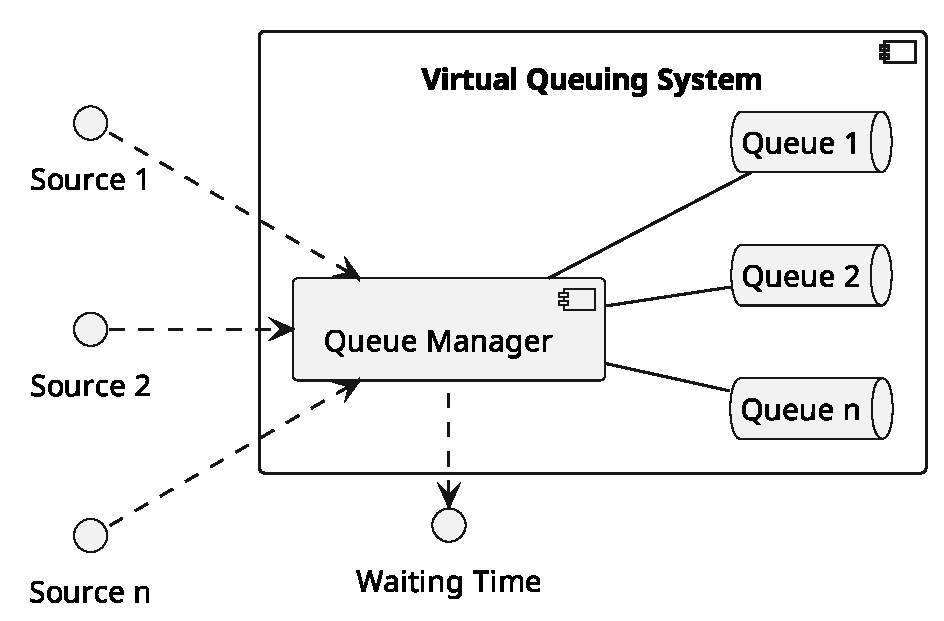
\includegraphics[width=0.6\textwidth]{img/virtual-queuing.eps}
	\caption{Component diagram showing the internal architecture of the \textit{Virtual Queueing} component.
	}
	\label{fig:virtual-queueing-arch}
\end{figure}

The Virtual Queueing System manages the waiting time of the people in the attractions queues. It could base its estimations on various sources such
as sensors (cameras, NFC, Bluetooth) or a button pressed on the visitor's wearable which communicates its presence in the queue. In fact, the best
way to implement this mechanism depends on the assumptions we could do about the context: in a Mirabilandia as a Micro City scenario every visitor
has a wearable where to enqueue themselves so there is no need to use high or low-budget sensors.

However, some sensors could be used to automatically detect corner case scenarios such as temporary roller coasters malfunctioning, bad weather etc.

\section{Planner}\label{sec:planner}

The Planner covers a main role in the overall system: the quality of experience of the user in the park depends also on it. The main goal of this component is to satisfy as much as possible the needs and preferences expressed by visitors and at the same time ensure the best possible experience.

\begin{figure}[H]
	\centering
	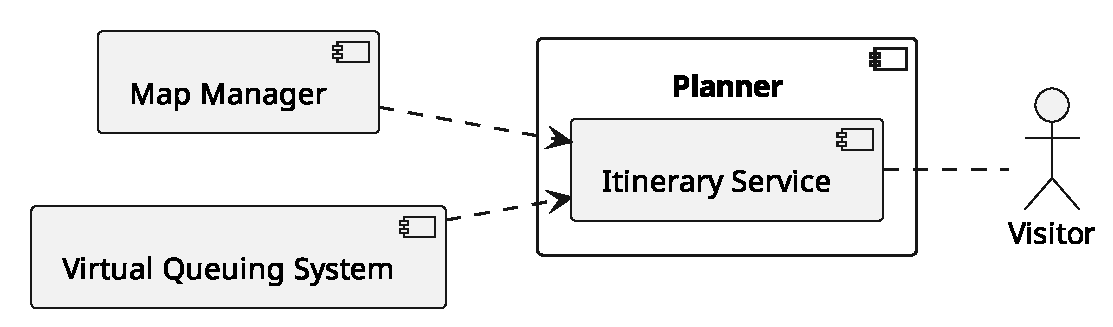
\includegraphics[width=0.7\textwidth]{img/planner.eps}
	\caption{Component diagram showing the internal architecture of the \textit{Planner} component.}
	\label{fig:planner-arch}
\end{figure}

In addition, park activities are as dynamic as park visitors are so it is easy to see that the needs of both parties may change in the process.
Therefore, it is appropriate to provide that the plans generated for visitors can change dynamically to adapt to changes in the environment. An
attraction may break down and therefore all plans that provided for the use of that ride must be adapted to the change. Again, overcrowding at an
attraction may be the reason why certain visitors' plans change to avoid excessively long queues.

From the above considerations, it is clear how the Planner needs to know in real-time: the queue status of each attraction, the preferences expressed
by each user, and the relative location within the park. Figure~\ref{fig:planner-arch} shows the dependencies that the Planner has with the rest of
the system, in particular, the information flows that the Planner needs to generate the plans are represented. The core of the \textit{Planner} is
the \textit{Itinerary Service} which collects all the information from the other components and provides the plans to each visitor.

\section{Visitors Manager}

The Visitor Manager is in charge of managing park visitor information. In particular, it is responsible for managing the visitor sign-up, the
preferences they express when accessing the park, as well as maintaining a whole range of information useful for user profiling. Moreover, the
Visitor Manager is responsible for managing the visitor's tickets, which are used to access the park and to pay for the services.

\begin{figure}[H]
	\centering
	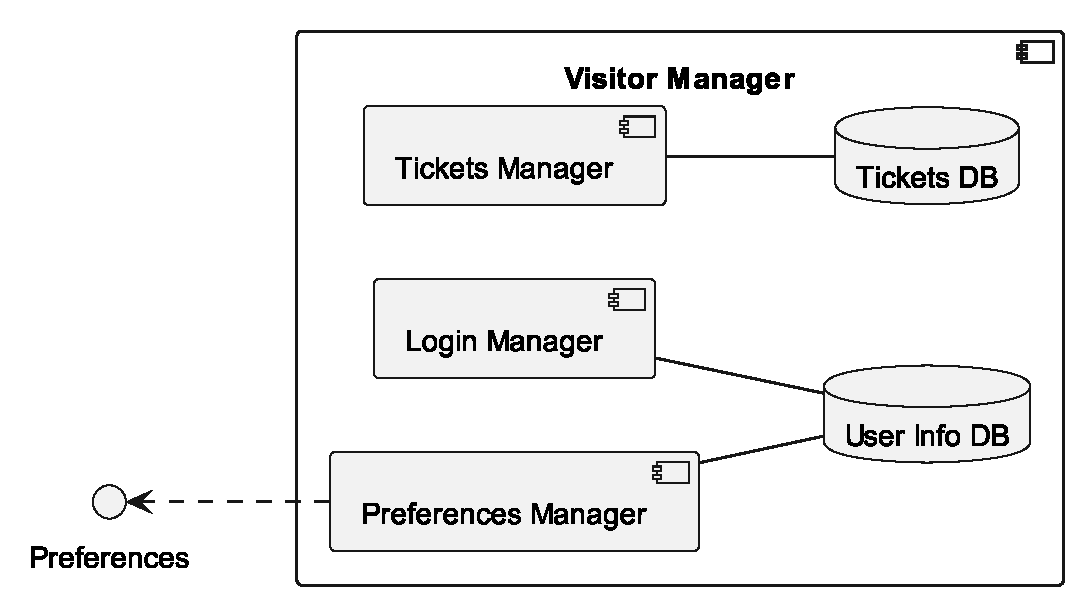
\includegraphics[width=0.7\textwidth]{img/visitor-manager.eps}
	\caption{Component diagram showing the internal architecture of the \textit{Visitor Manager} component.
	}
	\label{fig:visitor-manager-arch}
\end{figure}

The figure~\ref{fig:visitor-manager-arch} shows the internal architecture of the Visitor Manager component. The Visitor Manager is composed of three
main modules:

\begin{itemize}
	\item \textbf{Ticket Manager:} handles all the ticket-related operations like discounts, promotional offers, sales etc.
	\item \textbf{Login Manager:} handles all the login-related operations like sign-up, login, logout, password recovery etc.
	\item \textbf{Preferences Manager:} handles all the preferences related to a visitor like the preferred attractions, attractions to avoid, etc.
\end{itemize}

This component, through the data gathered from each visitor, provides the \textit{Recommender System} with the necessary information to provide the
best recommendations to the visitors.

Given the characteristics of this service and the operations it must perform, it is considered unnecessary to develop its version but rather to take
advantage of platforms already in the market that offers this kind of functionality (user management, user profiling, preference management, etc.).
For these reasons, it is not deemed necessary to examine this component further.

\section{Suitable technologies for Mirabilandia as a Micro City}
This chapter will examine in detail the technologies that are suitable for implementing the systems described above.
Particularly the techniques available for proximity marketing, crowd density estimation and people localization in indoor and outdoor environments.

\subsection{Proximity Marketing Technologies}\label{sec:proximity-marketing-technologies}
The situated Recommendation System broadcasts notifications to devices near a certain spot.
This is the same mechanism used for Proximity Marketing techniques and seems advantageous to use the same technologies to implement such a system since there is plenty of information in the literature regarding proximity marketing.
In the following section, we will examine some of the current technologies used to implement this kind of system.

\subsubsection{Proximity Marketing with Beacons}\label{sec:proximity-marketing-with-beacons}
Bluetooth low energy is one of the forms of Bluetooth which is designed for IoT-based applications. 
Bluetooth low energy is a standard of Bluetooth that does not provide a connection functionality (pairing) but instead, transmits signals continuously.
These signals can be detected by clients that are on the lookout for that particular beacon~\cite{muddinagiri2020implementation}.
Once a person with a device with Bluetooth turned on is near the beacon, the device collects the Beacon's ID, sends it to a server that retrieves the corresponding marketing information and returns it to the user with a message.

\subsubsection{Proximity Marketing using Wi-Fi}\label{sec:proximity-marketing-wifi}
Even though proximity-driven marketing systems have mostly been developed with the use of Bluetooth beacons~\cite{mndebele2017iot}, it is possible to
enable IoT-based proximity communication running as a service using network information, exploiting Wi-Fi. This offers better value than Bluetooth in
terms of efficiency and cost-effectiveness, as it can be used to implement IoT-based proximity solutions that run on existing infrastructure.
The detection of Wi-Fi networks already provides some data about location, namely information about proximity so proximity-based rules replace location
information, where Wi-Fi hot spots work as presence sensors~\cite{dmitry2013network}.

This paper~\cite{mndebele2017iot} for instance, presents a proximity marketing technique as a service (PMaas). The system targets people in a specific location
and delivers messages to their mobile devices via wireless connectivity technology as long as they remain in the specified location. Moreover, they
have to be connected to a particular network segment or specific access point. To do so, the system uses network information, i.e. the network name,
and GPS parameters derived from the position of the mobile device. The marketing messages are sent by a cloud-based platform to the eligible devices and a mobile app listens for messages applicable to the subscriber, while the subscriber is in the relevant proximity.

\subsection{Technologies for crowd density estimation}\label{subsec:sub-ghz-wireless-sensor-network-for-crowd-density-estimation}
In our context, crowd density estimation could be advantageous to redirect visitors toward less crowded places within the park. The classic approach
to obtaining this information is to make use of an optical camera-based system but the accuracy of these systems can be rather dependent on the
lighting conditions and they tend to require the availability of a large amount of computing power. Furthermore, the use of optical cameras raises
the spectre of privacy-related issues. A WSN-based system could potentially be used to simply avoid these issues~\cite{denis2018large}. In fact, the
use of sub-GHz frequencies could be the best decision, due to their increased range and penetration capabilities through objects, walls and human
individuals~\cite{denis2018large}. Moreover, this kind of transceivers, compared to the regular Wi-Fi, have a significant lower
power-consumption~\cite{fudickar2014comparing}.

As presented in~\cite{denis2018large}, they managed to show the feasibility of using a sub-GHz wireless network to estimate the density of
large-scale crowds calculating the mean RSS-differences within a WSN between an empty and an active environment and used them as input to a
probabilistic neural network. Whereas in~\cite{fudickar2014comparing}, showed that Sub GHz transceivers achieve significant lower RSS errors and are
less influenced by obstacles attenuations. Their localisation achieved ca. 1 m more accurate median error distances than the corresponding versions
that utilise Wi-Fi transceivers. In addition, the battery runtimes are extended by 48\% when using Sub GHz transceivers instead of Wi-Fi
transceivers.

\subsection{Technologies for visitors localization}\label{sec:technologies}
Visitors localization could be useful for both proximity marketing and calculating the number of people in a queue. Indoor localization could be
helpful in our context as there are restaurants, shops and some attractions (e.g.\
Reset\footnote{\url{https://www.mirabilandia.it/en/attivita/attrazioni/reset}}) not easily reached by the outdoor localization technologies.
Moreover, the accuracy of outdoor localization technologies (e.g.\ GPS) may not be enough accurate for instance for the prize games
area\footnote{\url{https://www.mirabilandia.it/en/attivita/attrazioni/altri-giochi-e-giochi-a-premio}} where the stands are located next to each
other.

To design and develop an effective technique for the location of visitors, the following constraints were considered:
\begin{itemize}
	\item The use of a custom device is not feasible since most people reject the use of a custom device. Using each visitor's device would be a better choice
	      because they do not have the impediment of an extra device and do not need any training to use it
	\item The use of dedicated hardware results in an extra cost that is difficult for both the amusement park and visitors to bear.
\end{itemize}

Some technologies identified for these purposes will be described taking into account the constraint defined above.

\subsubsection{Wi-Fi as outdoor localization system}\label{subsec:wi-fi-as-outdoor-localization-system}

Wi-Fi is a family of wireless network protocols, which are commonly used for local area networking of devices and Internet access, allowing the
nearby digital device to exchange data by radio waves.

To date, Wi-Fi is a technology that has been pervasively adopted and made accessible to anyone because of cost, ease of installation and
configuration.

Unlike other technologies such as the global positioning system (GPS), Wi-Fi was not designed to perform device and/or person location. However, by
exploiting ad-hoc techniques it is possible to leverage this tool to perform device localization. Finally, GPS does not always perform well in any
context: in closed environments or where the GPS signal cannot reach, localization using this technology is approximate or even impractical. Another
problem with GPS is its high power consumption, which is a serious challenge to battery-based mobile devices. To tackle the problems with GPS, many
researchers have proposed a series of alternative localization schemes, including cellular-based systems~\cite{ibrahim2010cellsense}, infrared-based
systems, ultrasonic-based systems, and radio frequency (RF)-based systems~\cite{bahl2000radar, youssef2002probabilistic}.

Many researchers have proposed a variety of different schemes for outdoor localization based on mobile devices. These schemes can be divided into two
groups: range-based and range-free methods.

\begin{itemize}
	\item \textbf{Range-based}: range-based methods are mainly based on relative distance, which can be obtained through measuring methods like
	      time-of-arrival (ToA), time difference of arrival (TDoA), or propagation model generated from RSSI value.
	\item \textbf{Range-free}: one of the most widely used range-free methods is the fingerprint localization method.
	      This method can be categorized into three types:
	      visual fingerprint-based localization, motion fingerprint-based systems, and signal fingerprint-based methods.
	      In our context, the latter is the most promising.
\end{itemize}

Signal fingerprint-based localization is widely used in places where a large number of Wi-Fi infrastructures are deployed. This method commonly
consists of an offline training phase and an online fingerprint matching phase. The goal of the first phase is to form a fingerprint database that
stores the correlation between \textit{Received Signal Strength} (RSS) from various \textit{Access Points}(APs) and fixed locations. The device's
location is determined at the matching stage. In this process, we use a matching algorithm to search the fingerprint in the database which has the
minimum difference with the device that needs to be located. The associated label is our estimated location.

In terms of effect, signal fingerprint-based localization can get fine-grained results. However, as any radio environment is dynamic: unpredictable
movements of the people or large unforeseen gatherings, alterations in the radio network itself, environmental effects such as a change in humidity
levels etc.~\cite{chaudhry2013indoor} Therefore, the RF values measured for location estimation at any given point in time may significantly deviate
from those stored in the database created at the training phase~\cite{chaudhry2013indoor}. As a result, the location estimation based on a static
database may be inaccurate. Also, the training phase needs a human operator (or a human-assisted machine) to thoroughly collect the RF context and
the location from which the context was collected. To tackle these problems, as suggested in~\cite{chaudhry2013indoor}, could be useful a system that
considers the NFC technology: reference points of precisely known locations are spread in the environment, marked by NFC tags, to build the database
of fingerprints around. This could improve the training phase and allows easy adaptation to environmental changes.

\subsubsection{Bluetooth as outdoor localization system}
Bluetooth is a data transmission standard for personal wireless networks. It provides a standard way to exchange information between devices through
a short-range frequency capable of detecting devices covered by the radio signal within about ten meters by putting them in communication with each
other.

Despite being a technology conceived more than 20 years ago, it boasts massive adoption in many contexts such as medical, industrial, and in recent
years the Internet of Things (IoT). This standard was designed to achieve low power consumption, short range and a low cost of production. Over the
years, there have been several updates to the protocol, aimed at improving on the one hand the efficiency of communication by enabling higher
transmission frequencies and on the other hand improving the energy efficiency of devices.

Bluetooth was not designed to perform localization functionality. However, it is possible to exploit certain features of the protocol to make a more
or less precise estimate of a device's location. In particular, the technique most used to achieve this is based on the signal strength identified by
the RSSI (Receives Signal Strength Indicator). Other techniques, such as fingerprint-based localization can be employed to estimate position.

With the RSSI-based technique, the RSSIs of all reachable Bluetooth devices are initially acquired, and through techniques of trilateration, the
location of the device is estimated.\\ Fingerprint-based techniques estimate the location by operating in two stages: the first is the training phase
that deals with building fingerprints, which is a record that associates a location with the RSSIs of beacons reachable from that point. The second
phase involves identifying the fingerprint that least deviates from the position where the device is at a given time, and the position associated
with that fingerprint determines the estimated position. Several projects and applications rely on these two techniques to estimate the position of a
device~\cite{mcconville2021vesta, samuel2021smart}.

The proliferation of location services for various IoT applications needs to detect device locations with very high accuracies, on the order of
centimeters. With the introduction of the Bluetooth 5.1 standard, a new feature called \textit{Direction Finding} enables pinpoint localization of
Bluetooth devices. This new localization feature provides two different options for positioning a Bluetooth device, namely Angle of Arrival (AoA) and
Angle of Departure (AoD) compared to the previous version that relies only on the received signal strength indication to localize a Bluetooth device.
To be more precise, the former technique allows a receiver equipped with a multi-antenna array to identify the angular position of a transmitter
based on the phase delay of the signal received from the transmitter; the latter allows the transmitting device with multiple antennas to transmit a
radio signal that permits the receiver to determine the directional angle to the transmitter.

\section{Identified technologies to make Mirabilandia a Micro City}
The technologies illustrated above can be used and applied to the Mirabilandia environment.
The following paragraphs have the objective to describe how this would be possible with a fair degree of detail.
\subsection{Planner strategies and considerations}
In this section, we are not going to provide an actual technology or algorithm for making plans, but rather we want to focus on what goals an
algorithm in charge of calculating the best plan should achieve based on various factors.

As mentioned in the section~\ref{sec:planner}, we should take into account three main aspects in building the optimal plan for each visitor: the
satisfaction of the guest's preferences, the maximization of the number of attractions visited and the minimization of the waiting time at each
attraction. The first two aspects may be similar but they are to be understood respectively as the ability to cater to user preferences and the
ability to maximize the number of attractions visited. The third aspect is the ability to minimize the waiting time at each attraction. The first two
aspects are related to the user's satisfaction, while the third aspect is related to the user's experience.

To evaluate the effectiveness of the plan, some metrics and indicators should be developed. Below is described a set of metrics and indicators that
could be useful in the evaluation of a plan.

\begin{itemize}
	\item \textbf{Completed Rides Indicator} (CRI): indicates the number of rides completed within one hour
	\item \textbf{Wandering Time Indicator} (WTI): indicates the quantity of time spent in the queues within one hour
	\item \textbf{User Satisfaction Indicator} (USI): indicates the number of rides completed in an hour but which were expressed as preferences by the visitor.
\end{itemize}

\begin{figure}[H]
	\centering
	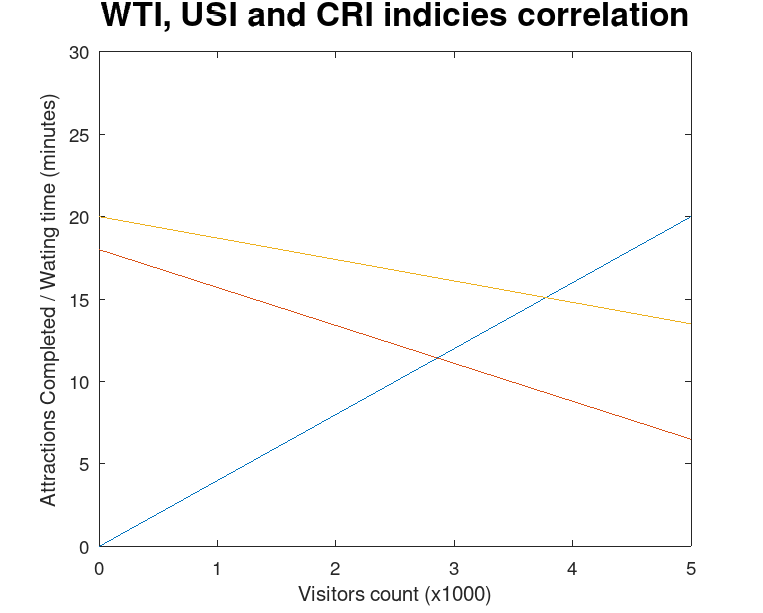
\includegraphics[width=0.8\textwidth]{img/indiciescorrelation.png}
	\caption{Correlation between the three indicators: \textit{CRI}, \textit{WTI} and \textit{USI}. This chart aims to give an empirical indication of the correlations between the three indicators. It's not based on any real data but it's a good way to understand the correlation between the three indicators.}
	\label{fig:indicies}
\end{figure}

In figure~\ref{fig:indicies}, is shown a possible correlation between the three indicators. The chart aims to provide an intuition about the trend of
the three indicators. We specify that it is not derived from any measurements nor available data, but in our opinion is a good way to get what the
indices mean.

The \textit{CRI} and \textit{USI} ad in opposition to the \textit{WTI}: if a plan is identified to provide only attractions that the user has
indicated, then the user is very likely to queue a lot and consequently increase the \textit{WTI} indicator. On the other hand, if a plan maximizes
the visitor's experience (increasing the \textit{CRI} indicator), then is quite likely that will be offered to them attractions that are not of their
interest, reducing the \textit{USI} indicator. The challenge behind the planning algorithm is to find a balance between these three indicators.

These indicators of course could be applied offline to evaluate the overall performance of the planner, but they could also be used online to adjust
in real-time the plan according to the environment changes. It is believed that a machine-learning approach could help the planning system to obtain
a better plan in real-time since it could learn from the past experiences of the visitors and adapt the plan accordingly. Moreover, due to the
complexity of the environment could not be feasible to tackle all possible scenarios, so a machine-learning approach could help to improve the plan.

\subsection{Localization techniques}
In this section, we will discuss the suitability of the localization techniques described in the previous section for Mirabilandia.

Given its size and organization, it comes naturally to think of Mirabilandia as a micro-city: streets, avenues and squares define the street network
that connects all the park's attractions and activities, just as it does for any full-scale city. The arrangement of buildings around the streets
also makes Mirabilandia a micro-city.

Given the similarities to a full-size city, we can assume with some degree of confidence that the amusement park environment is almost identical to
the city environment. Therefore, we assume that the noise and electromagnetic pollution are quite similar, and therefore all the considerations made
in the previous sections apply.

There is no definite information on the spread and coverage of Wi-Fi within the park, however, it is possible to assume that there is. Conversely, it
is by no means a given that there are Bluetooth devices that can act as beacons. In light of these considerations, we found that localization using
Wi-Fi is the most reasonable in terms of both effectiveness and cost of installation and configuration. The choice of using Wi-Fi as a technology to
support visitor tracking is based on three main considerations:

\begin{itemize}
	\item The cost of installation and configuration is relatively low since we have assumed a partially available infrastructure
	\item The spread of the technology is relatively wide, so any visitor's device support this technology.
	\item The literature about localization using Wi-Fi is relatively large, so it is feasible to use this technology.
\end{itemize}

In this scenario, Bluetooth technology has been discarded because of the low signal range and this would force the installation of many more devices
than would be needed by taking advantage of Wi-Fi; also because in outdoor environments Bluetooth provides lower guarantees in terms of signal
stability and this results in possible inaccuracies in location estimation. Finally, the introduction of the 5.1 standard is fairly new, and while it
is not a problem in terms of adoption, there are still no comprehensive studies on its effectiveness in amusement park-like environment.

Below we will illustrate a possible technique for implementing park visitor tracking by exploiting Wi-Fi as a supporting technology. The development
of this technique is based on work done by~\cite{du2018hybrid}~and~\cite{chaudhry2013indoor}.

The localization scheme consists of three main phases:

\begin{itemize}
	\item \textbf{Training phase:} in this phase, the system collects the RSSI values of the Wi-Fi APs in the park and associates them with a
	      physical position. This phase could be performed by a human operator or a human-assisted machine
	\item \textbf{Tiling phase:} in this phase the system divides the park into a grid of tiles and caches the values belonging to it
	\item \textbf{Inference phase:} in this phase the system calculates the dissimilarity between the collected patterns and the sample
	      patterns in the database built before. The location of the fingerprint with the minimum difference will be selected as an estimation for the
	      location of the device.
\end{itemize}

The \textit{training phase} is the most important and challenging phase of the scheme. It is the phase in which the system collects the RSSI values
of the Wi-Fi APs in the park and associates them with a physical position. The accuracy of this phase is crucial: a wrong position in a fingerprint
could result in inaccurate location estimation. The collection of the fingerprint database could be done in several ways: by a human operator, which
walking around the park collects the RSSI values of the Wi-Fi APs and associates them with a physical position, creating a fingerprint record.
Alternatively, a fleet of robots (like drones) could be used to collect the RSSI values and associate them with a physical position. This scenario is
ambitious but could be faster and less error-prone than the human ones.

The \textit{tile phase} consists of a series of optimizations exploited by the \textit{inference phase} to reduce the inference time. The map is
divided into regions, each containing fingerprints of the locations contained in it. In this way, it is not required to use the entire fingerprint
database, but only the region (or regions) of interest. Finally, each tile can be cached for additional performance improvements during the inference
phase. Determining which tile should be used for the inference step is not an easy task. Choosing the wrong tile may result in an incorrect position
estimate. At the same time, it is particularly inefficient to estimate the position by leveraging the entire fingerprint database. For this reason, a
sensor-assisted matching method can restrict the matching operation in a small space through sensor information including direction and travel
distance. The current location can be calculated from an initial location, which can be taken from the GPS, for example. The distance and direction
can be estimated using the dead reckoning~\footnote{\url{https://en.wikipedia.org/wiki/Dead_reckoning}} method with built-in inertial sensors like
accelerometer, gyroscope, and compass. Given the longitude and latitude of the start point, the distance and bearing from the start point, and the
destination point can be calculated using the Haversine formula~\footnote{\url{https://en.wikipedia.org/wiki/Haversine_formula}}. In this way, a
subset of the local fingerprint database cache can be obtained.

The \textit{inference phase} is the most important phase of the scheme. It is the phase in which the system calculates the position of the device.
Let's denote by $f = {r_1, r_2, \ldots, r_n}$ a \textit{fingerprint} record where $r_i$ represents the RSS value of captured AP and $n$ the number of
APs in the fingerprint record. Let's calculate the dissimilarity between two fingerprints based on the RSSI difference. Denote with $\sigma_i = | r_i
	- r^{'}_{i}|$ the difference of fingerprints $f^{'}$ and $f$ at each $A_i$ where $A_i \in A$ where $A$ is the fingerprint database. Since two
fingerprints may contain a different set of APs, the access point $A_i$ may appear in $f$ but does not appear in $f^{'}$. For this situation, we
assume the signal strength is weak and let the missing value equal to $-100$. The dissimilarity between $f$ and $f^{'}$ is calculated via the
following formula:

\begin{equation}
	\eta(f, f^{'}) = \sqrt{\sum_{i=0}^{p} \sigma_i^{2}}
	\label{eq:dissimilarity}
\end{equation}

where $p = | A \cup A^{'} |$

The location is calculated via the sample with minimum dissimilarity by comparing all samples stored in the fingerprint database $F$ with the query
fingerprint $f$.

\begin{equation}
	f^{*} = \arg \min_{f_i \in F} \ \eta(f, f_i)
	\label{eq:min-dissimilarity}
\end{equation}

$L(f^{*})$ is the corresponding location of $f^{*}$ which represents the estimated place.

As can be seen from formula~\ref{eq:min-dissimilarity}, the iteration over all fingerprints cannot scale at all: the time needed to iterate all the
fingerprints are proportional to the number of them. In large maps, the number of fingerprints could become very huge degrading the inference time.
It is in this situation that tiling improves performance due to dimension reduction; this reduction is determined by the $k$ factor, where $k$ is the
number of tiles of the map.

\begin{figure}[H]
	\centering
	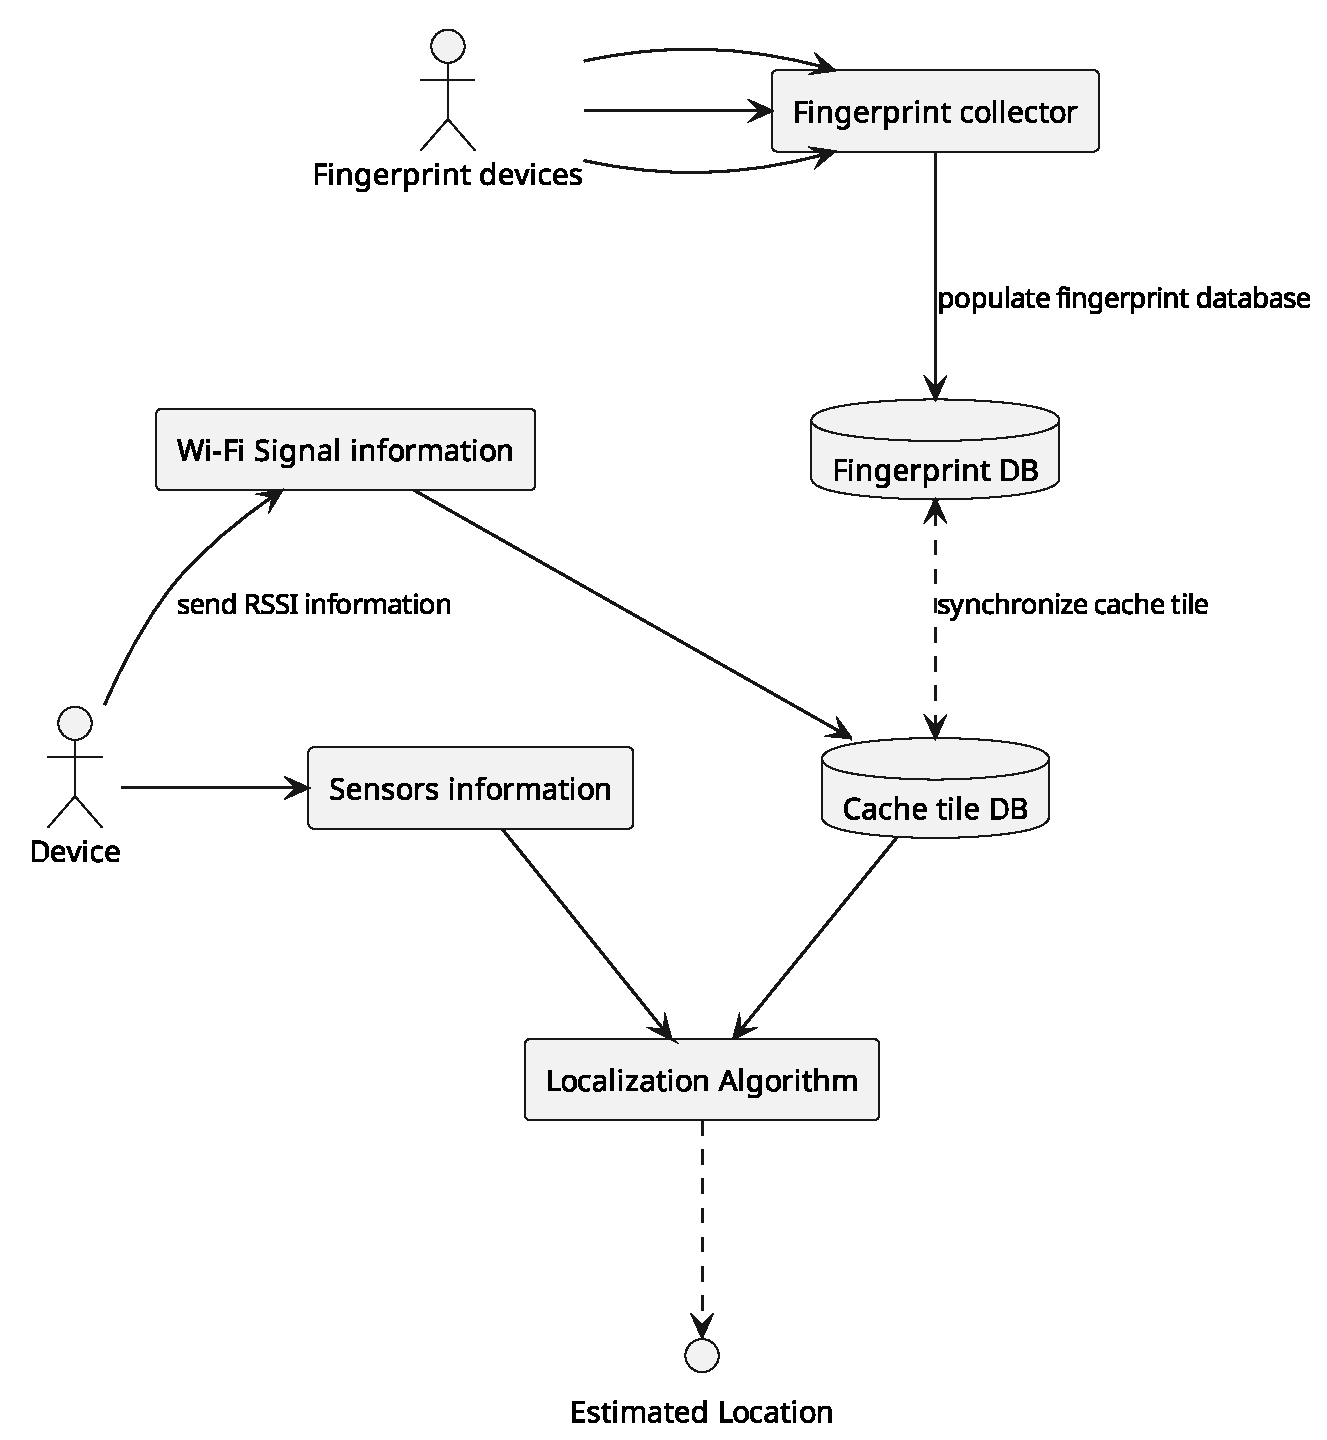
\includegraphics[width=0.7\textwidth]{img/fingerprint-schema.eps}
	\caption{Main steps in the proposed schema for Wi-Fi fingerprint-based localization technique.}
	\label{fig:fingerprint-schema}
\end{figure}

In figure~\ref{fig:fingerprint-schema} are summarized the steps for the localization based on Wi-Fi.

The adoption of this technique leads to several advantages:
\begin{itemize}
	\item The accuracy of the localization is improved compared with the GPS one~\cite{du2018hybrid}
	\item The power consumption needed to implement this system is sensible lower than the GPS~\cite{du2018hybrid}
	\item The flexibility of this technique enables the computation of the location either on the device or on the server.
\end{itemize}

We believe that Wi-Fi-based calculation of visitor location within the amusement park is a promising solution in terms of both effectiveness (more
accurate location and lower consumption) and costs instead of using a traditional system like GPS.

\section{Deployment strategy for a real case scenario}
In this section, we will examine a possible deployment strategy for the proposed system. In particular, we will take into account all the pros and
cons of a full cloud solution, a full edge solution, and a hybrid solution.

\subsection{Edge computing vs Cloud computing}
First, it's important to understand that cloud and edge computing are different, noninterchangeable technologies that cannot replace one another.
Edge computing is used to process time-sensitive data, while cloud computing is used to process data that is not time-driven. While cloud computing
is designed to provide high availability and on-demand scaling, the latency introduced by the communication could increase a lot the response time.
Edge computing is designed to reduce latency by processing data locally. The main advantage of edge computing is the reduction of latency, but it has
some drawbacks. The main one is the lack of scalability. Edge computing is not designed to scale, so it's not possible to add more nodes to increase
processing power. Another drawback is the high cost of the infrastructure.

Thus, we can conclude that the cloud has the advantages of providing high computing power and scaling on demand; on the other hand, it has as its
main disadvantage the high delay in communication between devices and the cloud itself. On the other hand, the edge has the disadvantage of having
limited computational resources and higher utilization costs but has the advantage of having very fast communication times with devices.

\subsection{Fog computing}
Traditional cloud-based IoT systems are challenged by the large scale, heterogeneity, and high latency witnessed in some cloud ecosystems. 
Fog computing is a possible solution as it's a distributed computing paradigm that extends cloud computing to the edge of the network:
it allows the decentralization of applications, management, data analytics, etc. into the network itself.

This model enables ubiquitous access to a shared continuum of scalable computing resources.
The deployment of distributed, latency-aware applications and services is facilitated and consists of fog nodes (physical or virtual), residing between smart end devices and centralized (cloud) services.
The fog nodes are context-aware and support a common data management and communication system.
They can be organized in clusters - either vertically (to support isolation), horizontally (to support federation), or relative to fog nodes' latency distance to the smart end devices. Fog computing minimizes the request-response time from/to supported applications, and provides, for the end-devices, local computing resources and, when needed, network connectivity to centralized services~\cite{iorga2018fog}.

This is an interesting model for some components of our use case.

\subsection{Hybrid architecture: edge, cloud and fog}
The advantages of one approach and the other do not by themselves justify the choice of one or the other. Rather, we believe that the adoption of all the technologies leads to a concrete advantage in the realization of Mirabilandia as a Micro City.

We then go on to analyze the requirements of each system component described in section~\ref{sec:mira-microcity}, and for each one, we will identify whether it is best implemented in a cloud, edge or fog context.

\subsubsection{Recommendation System deployment strategy}
As we previously said in other sections, our situated Recommendation System is similar to a Proximity Marketing system.
Thus, the deployment strategy could use some state-of-the-art technologies that can be found in the literature regarding this topic.
Mirabilandia has a large number of visitors every day and current technology infrastructures and architectures need to be designed to process in real-time the great amount of information data that is being made available from such several devices with a so high concentration.

\subsubsection{Virtual Queueing System deployment strategy}

\subsubsection{Visitor Manager deployment strategy}
Concerning the \textit{Visitor Manager} component, this has no particular constraints either in terms of computational complexity or latency in
communications; dealing mainly with managing user master data and their preferences in addition to being in charge of ticket sales, this component
can exist in a cloud context or an external CRM can be leveraged.

\subsubsection{Planner deployment strategy}
The \textit{Planner} is responsible for managing the plans for each park visitor. This task requires fairly high computational capabilities since the
plan can evolve. Although itinerary management is a relevant aspect, the speed of plan generation is not considered of primary importance. Even if
the updated plan is propagated to visitors within a few seconds or a few tens of seconds, it is not believed to infect the overall visitor
experience. Given these requirements, it is believed that a cloud solution can adhere well to the needs of this component. The choice of the cloud is
further strengthened by the fact that the computational requirements can vary quite a bit over time: there may be times of the year when the
attendance of people at the amusement park is rather limited, so the plans to be calculated turn out to be fewer in number and therefore less
computational capacity is required. Conversely, on the other hand, at peak times visitor turnout requires significantly increased computational
capacity to meet the demands. The dynamism with which resources can be allocated or de-allocated is something that the cloud natively handles, thus
representing the optimal solution for implementing such a service.

\subsubsection{Map Manager deployment strategy}
The \textit{Map Manager} is responsible for maintaining information on the location of each visitor within the park. It is the component that has the
most interaction with visitor devices and the one that requires a near-real-time operation. This component requires component-device communication to
be as fast as possible to calculate the corresponding location. In this context, the computational complexity required for position computation is
not very high, but low latency in communications is required. For this reason, an edge solution would be ideal to implement such a system. To further
reduce the latency in communication, it is possible to think of a hybrid scenario: initially, it is the device that, using the same algorithm,
estimates its position within the park and directly sends the position information to the service. In this way the \textit{Map Manager} acts as an
aggregator of information that it then makes available to the other services. If the device fails to compute the position promptly or due to other
factors it is deemed that the computation should be done offline, then the device reverts to operating as described above, i.e., it sends only the
information that is useful for making the position computation, which, however, will be done by the \textit{Map Manager}. In this way, one can
opportunistically determine where it is best to perform the computation of the position estimate.

% TODO: deployment architecture image!

\subsection{Situated Recommendation system}
To implement the situated Recommendation system in Mirabilandia we could assume that the technology for detecting the presence of a visitor in a certain spot isn't crucial.

In fact, could be sufficient to associate the location of the visitor with an ID and the ID with an action. Then the system generates a recommendation for the user based on the action, the position and the visitor's information.

This way, the "situated" part of the system can be implemented in a very simple way.

The system workflow is shown in Figure~\ref{fig:situated-recommendation}.

\begin{figure}[H]
	\centering
	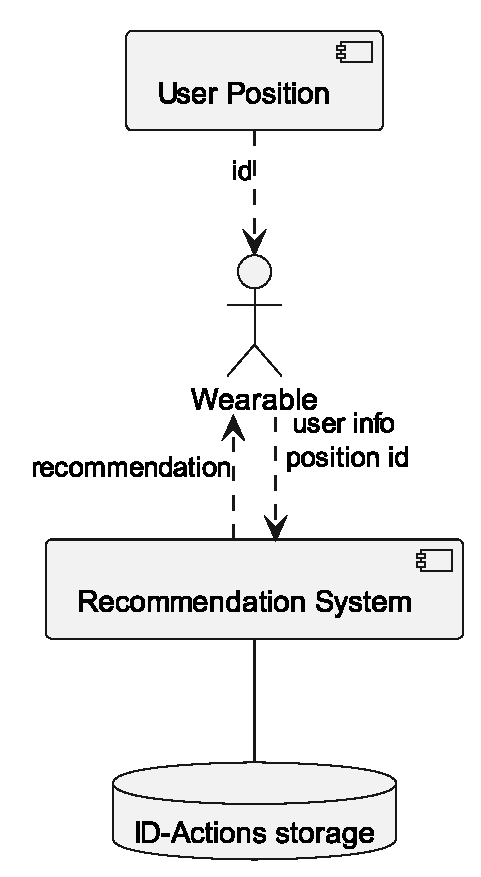
\includegraphics[width=0.3\textwidth]{img/situated-recommendation.eps}
	\caption{Situated Recommendation System components.}
	\label{fig:situated-recommendation}
\end{figure}
